First suggested in \cite{Granade:2012kj} and since developed \cite{wiebe2014qhlpra, Wiebe:2014qhl} 
    and implemented \cite{wang2017experimental,gentile2020learning}, 
\gls{qhl} is a machine learning algorithm for the optimisation of a given Hamiltonian parameterisation 
    against a quantum system whose model is known apriori. 
Given a target quantum system \gls{q} known to be described by some Hamiltonian $\hat{H}(\vec{\alpha})$, 
    \gls{qhl} optimises $\vec{\alpha}$.
This is achieved by interrogating \gls{q} and comparing its outputs against proposals $\vec{\alpha}_p$. 
In particular, an experiment is designed, consisting of an input state, $\ket{\psi}$, and an evolution time, $t$.
This experiment is performed on \gls{q}, whereupon its measurement yields the datum $d \in \{0, 1\}$, 
    according to the expectation value $\left| \bra{\psi} e^{-i \ho t} \ket{\psi} \right|^2$. 
Then on a trusted (quantum) simulator, proposed parameters $\vec{\alpha}_p$ are encoded to the 
    known Hamiltonian, and the same probe state is evolved for the chosen $t$ and projected on to $d$, 
    i.e. $\left| \bra{d} e^{-i \hat{H}(\vec{\alpha}_p) t } \ket{\psi} \right|^2 $ is computed.
The task for \gls{qhl} is then to find $\vec{\alpha}^{\prime}$ for which this quantity 
    is close to 1 for all values of $(\ket{\psi}, t)$, 
    i.e. the parameters input to the simulation produce dynamics consistenst with those measured from \gls{q}.
\par 

The procedure is as follows. 
A \emph{prior} probability distribution $\pra$ of dimension $\left| \al \right|$ 
    is initialised to represent the constituent parameters of $\al$. 
$\pra$ is typically a multivariate normal (Gaussian) distribution; 
    it is therefore necessary to pre-suppose some mean and width for each parameter in $\al$. 
This imposes prior knowledge on the algorithm whereby the programmer must decide the range in 
    which parameters are \emph{likely} to fit:
    although \gls{qhl} is generally robust and capable of finding parameters outside of this prior,
    the prior must at least capture the order of magnitude of the target parameters. 
An example of imposing such domain-specific prior knowledge is, 
    when choosing the prior for a model representing an $e^-$ spin in a \gls{nv} centre,
    to select $GHz$ parameters for the electron spin's rotation terms, and $MHz$ terms 
    for the spin's coupling to nuclei, as proposed in literature. 
It is important to understand, then, that \gls{qhl} removes the prior knowledge 
    of precisely the parameter representing an interaction in \gls{q}, but does rely on a ball-park estimate thereof from which to start. 
\par 

In short, \gls{qhl} samples parameter vectors $\al_p$ from $\pra$, 
    simulates experiments by computing the \emph{likelihood} $\left| \bra{d} e^{-i \hat{H}(\al_p)t} \ket{\psi} \right|^2$
    for experiments ($\ket{\psi}, t)$ designed by a \gls{qhl} heuristic subroutine, 
    and iteratively improves the probability distribution of the parameterisation $\pra$ 
    through standard \emph{Bayesian inference}. 
A given set of $(\ket{\psi}, t)$ is called an experiment, since it corresponds to preparing, evolving and measuring \gls{q} 
once\footnote{experimentally, this may involve repeating a measurement many times to determine a majority result and to mitigate noise}. 
\gls{qhl} iterates for $\Ne$ experiments. 
The parameter vectors sampled are called \emph{particles}: there are $\Np$ particles used per experiment. 
Each particle used incurs one further calculation of the likelihood function -- 
    this calculation, on a classical computer, is exponential in the number of qubits of the model under consideration
    (because each unitary evolution relies on the exponential of the $2^n \times 2^n$ Hamiltonian matrix of $n$ qubits). 
Likewise, each additional experiment incurs the cost of calculation of $\Np$ particles, 
    so the total cost of running \gls{qhl} for a single model is $\propto \Ne \Np$.
It is therefore preferable to use as few particles and experiments as possible, 
    though it is important to include sufficient resources that the parameter estimates have the opportunity to converge. 
Access to a fully operational, trusted quantum simulator admits an exponential 
    speedup by simulating the unitary evolution instead of computing the matrix exponential classically.
\par 

\section{Bayes Rule}
Bayes' rule is used to update a probability distribution describing hypotheses, $\Pr(\textrm{hypothesis})$, when presented with new information (data).
That is, the probabilty that a hypothesis is true is replaced
    by the initial probability that is was true, $\Pr(\textrm{hypothesis})$, multiplied by 
    the \gls{likelihood} that the new data would be observed were that hypothesis true, 
    $\Pr(\textrm{data} | \textrm{hypothesis})$, 
    normalsied by the probability of observing that data in the first place, $\Pr(\textrm{data})$. 
It is stated as
    \begin{equation}\label{eqn:bayes_rule}
        \Pr( \textrm{hypothesis} | \textrm{data} ) = 
        \frac{ \Pr( \textrm{data} | \textrm{hypothesis} ) \times \Pr( \textrm{hypothesis} )}{ \Pr(\textrm{data})}.
    \end{equation}
\par 
We wish to represent our knowledge of Hamiltonian parameters with a distribution, $\Pr(\al)$:
    in this case hypotheses $\al$ attempt to describe data, $\expdata$, measured from the target quantum system,  
    from a set of experiments $\expset$, so we can rewrite Bayes' rule as 
\begin{equation}\label{eqn:qhl_bayes_rule}
    \Pr(\vec{\alpha} | \expdata; \expset) = \frac{\Pr(\expdata| \vec{\alpha}; \expset) \ \Pr(\vec{\alpha})}{\Pr(\expdata|\expset)}.
\end{equation}

We can then discretise \cref{eqn:qhl_bayes_rule} to the level of single particles (individual vectors in the parameter space), sampled from $\Pr(\al)$:
\begin{equation}\label{eqn:particle_bayes_rule}
    \Pr(\al_p | d; e) = \frac{ \Pr(d | \ \al_p; \ e ) \ \Pr(\al_p) } {\Pr(d | e)}
\end{equation}

where 
\begin{easylist}[itemize]
    & $e$ are the experimental controls of a single experiment, e.g. evolution time and input probe state;
    & $d$ is the datum, i.e. the binary outcome of measuring \gls{q} under conditions $e$;  
    & $\al_p$ is the \emph{hypothesis}, i.e. a single parameter vector, called a particle, sampled from $\Pr(\al)$;
    & $\Pr(\al_p | d; e)$ is the \emph{updated} probability of this particle following the experiment $e$, 
        i.e. accounting for new datum $d$, the probability that $\al=\al_0$;
    & $\Pr(d |\al_p ; e)$ is the likelihood function, 
        i.e how likely it is to have measured the datum $d$ from the system assuming $\al_p$ are the true parameters
        and the experiment $e$ was performed; 
    & $\Pr(\al_p)$ is the probability that $\al_p=\al_0$ according to the prior distribution $\Pr(\al)$, 
        which we can immediately access; 
    & $\Pr(d|e)$ is a normalisation factor, the chance of observing $d$ from experiment $e$ irrespective of the underlying hypothesis.
\end{easylist}

In order to compute the updated probability for a given particle, then, all that is required is a value for the likelihood function.
This is equivalent to the expectation value of projecting $\ket{\psi}$ onto $d$, after evolving $\hat{H}(\al_p)$ for $t$, i.e. 
\begin{equation}
    \label{eqn:likelihood}
    \Pr(d | \al; e) = \left| \bra{d} e^{-i \hat{H}(\al_p)t} \ket{\psi} \right|^2,   
\end{equation}
    which can be simulated clasically or using a quantum simulator (see \cref{sec:likelihood}). 
It is necessary first to know the datum $d$ (either 0 or 1) which was projected by \gls{q} under real experimental conditions. 
Therefore we first perform the experiment $e$ on \gls{q} 
    (preparing the state $\ket{\psi}$ evolving for $t$ and projecting again onto $\bra{\psi}$)
    to retrieve the datum $d$. 
$d$ is then used for the calculation of the likelihood for each particle sampled from $Pr({\al})$. 
Each particle's probability can be updated by \cref{eqn:particle_bayes_rule}, 
    allowing us to redraw the entire probability distribution -- i.e. we compute a \emph{posterior} probability distribution
    by performing this routine on $\Np$ particles. 


\section{Sequential Monte Carlo}\label{sec:smc}
\begin{figure}
    \setcounter{subfigure}{0}

    \centering
    \subfloat{
        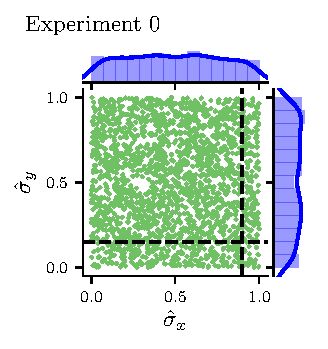
\includegraphics{algorithms/figures/smc_demo/epoch_0.pdf}
    }
    \subfloat{
        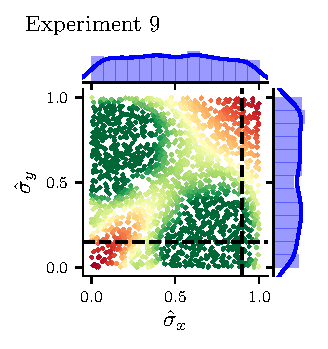
\includegraphics{algorithms/figures/smc_demo/epoch_9.pdf}
    }
    \subfloat{
        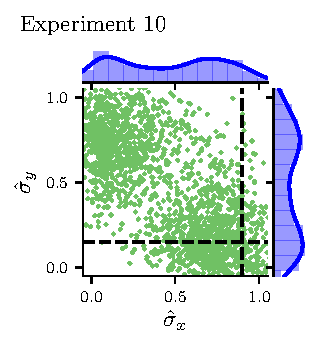
\includegraphics{algorithms/figures/smc_demo/epoch_10.pdf}
    }
    % \hspace{0mm}
    
    \subfloat{
        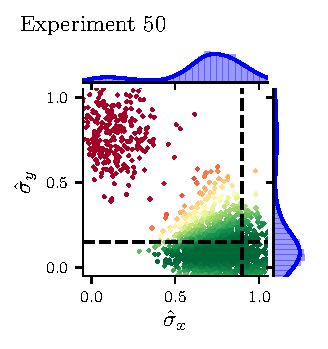
\includegraphics{algorithms/figures/smc_demo/epoch_50.pdf}
    }
    \subfloat{ 
    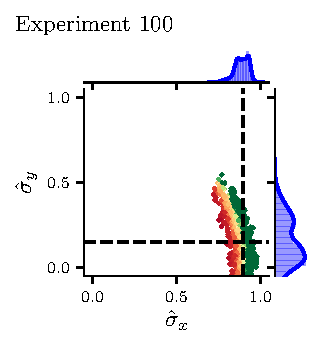
\includegraphics{algorithms/figures/smc_demo/epoch_100.pdf}
    }
    \subfloat{ 
    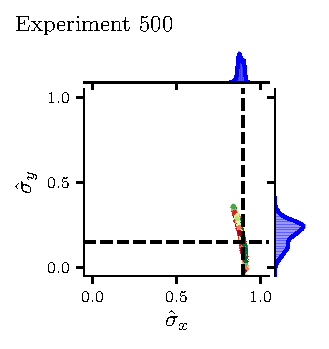
\includegraphics{algorithms/figures/smc_demo/epoch_500.pdf}
    }
    % \hspace{0mm}
    \subfloat{
        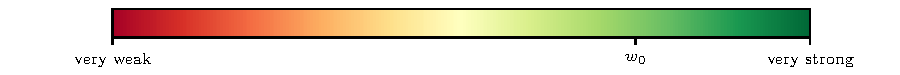
\includegraphics{algorithms/figures/smc_demo/cbar.pdf}
    }
    \caption[Quantum Hamiltonian learning via sequential Monte carlo]{
    \Acrfull{qhl} via \acrfull{smc}. 
    The studied model has two terms, $\{\sx, \sy\}$ with true parameters $\alpha_{x}=0.9, \alpha_y=0.15$ (dahsed lines), 
        with $\Ne=500, \Np=2000$. 
    Crosses represent particles, while the distribution $\Pr(\alpha_p)$ for each 
        parameter can be seen along the top and right-hand-sides of each subplot. 
    Both parameters are assigned a uniform probability distribution $\mathcal{U}(0,1)$, representing our prior knowledge of the system. 
    \textbf{(a), }\gls{smc} samples $\Np$ particles from the initial joint probability distribution, 
        with particles uniformly spread across the unit square, each assigned the starting \emph{weight} $w_0$. 
        At each experiment $e$, each of these particles' likelihood is computed according to \cref{eqn:particle_bayes_rule}
        and its weight is updated by \cref{eqn:qhl_weights}.
    \textbf{(b),} after 9 experiments, the weights of the sampled particles are sufficintly informative that we know we can 
        discard some particles while most likely retaining the true parameters. 
    \textbf{(c),} \gls{smc} resamples according the current $\Pr(\al)$, 
        i.e. having accounted for the experiments and likelihoods observed to date, 
        a new batch of $\Np$ particles are drawn, and each reassigned weight $w_0$, 
        irrespective of their weight prior to resampling.  
    \textbf{(d, e),} Afer further experiments and resamplings, \gls{smc} narrows $\Pr(\al)$ to a region around the true parameters. 
    \textbf{(f),} The final \emph{posterior} distribution consists of two narrow distributions centred on $\alpha_x$ and $\alpha_y$. 
    }
    \label{fig:qhl_smc}
\end{figure}

In practice, \gls{qhl} samples from and updates $\Pr(\al)$  via \gls{smc}.
\gls{smc} samples the $\Np$ particles from $\Pr(\al)$, and assigns each particle a weight, $w_0 = 1/\Np$.
Each particle corresponds to a unique position in the parameters' space, i.e. $\al_p$.
Following the calculation of the likelihood, $\Pr(d | \al_p; e)$, 
    the weight of particle $p$ are updated by \cref{eqn:qhl_weights}.
\begin{equation}\label{eqn:qhl_weights}
    w_p^{new} = \frac{\Pr(d | \al_p; e) \times w_p^{old} } { \sum\limits_{p} w_p \Pr(\al_p | d; e) }
\end{equation}

In this way, strong particles (high $\Pr(d | \al_p; e)$) have their weight increased, 
    while weak particles (low $\Pr(d | \al_p; e)$) have their weights decreased, 
    and the sum of weights remains normalised. 
Within a single experiment, the weights of all $\Np$ particles are updated thus:
    we \emph{simulataneously} update sampled particles' weights as well as $\Pr(\al)$. 
This iterates for the following experiment, using the \emph{same} particles: 
    we do \emph{not} redraw $\Np$ particles for every experiment.
Eventually, the weights of most particles fall below a threshold, $r_t$, 
    meaning that only that fraction of particles have reasonable likelihood of being $\al_0$.
At this stage, \gls{smc} \emph{resamples}, i.e. selects new particles, according to the updated $\Pr(\al)$,
    according to the Liu-West resampling algorithm \cite{liu2001combined}.
Then, the new particles are in the range of parameters which is known to be more likely, 
    while particles in the region of low-weight are effectively discarded. 
Usually, we set $r_t=0.5$, although this \gls{hyperparameter} can have a large impact 
    on the rate of learning, so can be optimised in particular circumstances, 
    see \cref{fig:param_learning_vary_particles}.
This procedure is easiest understood through the example presented in \cref{fig:qhl_smc}, 
    where a two-parameter Hamiltonian is learned starting from a uniform distribution. 


\section{Likelihood}\label{sec:likelihood}
The fundamental step within \gls{qhl} is the calculation of \gls{likelihood} in \cref{eqn:particle_bayes_rule}. 
The core of this learning algorithm is that this \gls{likelihood} can be retrieved from the Born rule, 
    although in principle \emph{any} valid likelihood function can fulfil this equation, 
    provided the calculation of the likelihood captures the probabilty that the present hypothesis produced the present datum.

In general, it is not always possible to derive the analytical likelihood, 
    especially in cases where we wish to vary the \gls{probe}.
When \cref{eqn:likelihood} can be computed classically, 
    \gls{qhl} relies on \gls{cle}, i.e. involving the exponential calculation of \cref{eqn:likelihood}, 
    whereas \gls{qle} uses the same likelihood function computed on a quantum simulator; 
    this is the sole application of quantum simulators in this protocol and indeed the remainder of this thesis. 
Access to such hardware, operating perfectly, would provide exponential speedup in the calculation of this term, 
    rendering both \gls{qhl} and the wider \gls{qmla} formalism scalable,
    although in this thesis we do not implement \gls{qle} so everything can be viewed as \gls{cle}. 
\gls{qle} was implemented in \cite{wang2017experimental}. 
\par 

We adopt notation used by QInfer, which \gls{qmla} for the likelihood estimation stage \cite{qinfer-1_0}. 
The expectation value for a the unitary operator is given by
\begin{equation}\label{eqn:pr0}
    \Pr(0) =  |\bra{\psi} e^{-i \hat{H}_p t} \ket{\psi}|^2  = l(d=0 | \hat{H}_p; e), 
\end{equation}
    i.e. the input basis is assigned the measurement label $d=0$, and this quantity is the probability 
    of measuring $d=0$, i.e. measuring the same state as input. 
However, we assume a binary outcome model, 
    i.e. that the system is measured either in $\ket{\psi}$ (labelled $d=0$), or it is not ($d=1$);
    the likelihood for the latter case is
\begin{equation}\label{eqn:pr1}
    \Pr(1) = l(d=1 | \hat{H}_p; e) = \sum_{\{\ket{\psi_{\perp}}\}} | \bra{\psi_{\perp}} e^{-i \hat{H}_p t} \ket{\psi}  |^2 = 1 - \Pr(0).
\end{equation}
\par 
Usually we will refer to the case where \gls{q} is projeced onto the input state $\ket{\psi}$, 
    so the terms \emph{likelihood}, \emph{expectation value} and \emph{$\Pr(0)$} are synonymous, 
    unless otherwise stated. 


\subsection{Interactive Quantum Likelihood Estimation}\label{sec:iqle}
An important extension to \gls{qle} is \gls{iqle}, 
    which follows \gls{smc} but uses an alternative \gls{likelihood} function in order to 
    overcome some of its inherent challenges \cite{Wiebe:2014qhl}. 
Two almost identical Hamiltonians will diverge after exponentially small evolution time \cite{jalabert2001environment}.
This is problematic for \gls{qhl} because it relies on the likelihood function which is built on the assumption 
    that increasing accuracy of $\ha$ approximating $\ho$ should result in rising likelihood;
    this result indicates that even extremely accurate approximations become unreliable after very short evolution times. 
Coupled with the result that small time experiments are uninformative \cite{wiebe2015quantum}, 
    this observation demands exponentially many measurements to approximate the exponentially small likelihoods, 
    rendering the approach inefficient. 
\par 
The \gls{le} is the measure of the revival resulting from an imperfect time-reversal operation implemented after the standard time evolution. 
The reversal operation corresponds to some Hamiltonian, $\hat{H}_{-}$, which is seen as an attempt to un-do the evolution
    according to the original Hamiltonian, $\hat{H}_{+}$. 
As such we say that $\hat{H}_{-}$ is evolved for $-t$, so its unitary is $e^{-i \hat{H}_{-}(-t)}$ after $\hat{H}_{+}$ is evolved for $t$. 
The \gls{le} can be written and characterised as 
\begin{align}
    \label{eqn:loschmidt_echo}
    M(t) = \absval{ \braket{ \psi | e^{+i\hat{H}_{-} t} e^{-i \hat{H}_{+} t} | \psi} }^2 \sim 
    \begin{cases}
        1 - \mathcal{O}(t^2),  & t \leq t_c \\
        e^{-\mathcal{O}(t)}, & t_c \leq t \leq t_{s} \\
        \nicefrac{1}{\| \hat{H} \|}, & t \geq t_{s}
    \end{cases}
\end{align}
    where $\hat{H}_{-}, \hat{H}_{+}$ are backward and forward time evolutions respsectively, which are assumed almost identical;
    $\|\hat{H}\|$ is their dimension, and $t_c, t_{s}$ are bounds on the evolution time marking the transition between the 
    \emph{parabolic decay}, \emph{asymptotic decay} and \emph{saturation} of the echo \cite{goussev2012loschmidt}. 
In effect, the \gls{le} gaurantees that if $\hat{H}_{-} \not\approx \hat{H}_{+}$, then $M(t) \ll 1$, 
    while $\hat{H}_{-} \approx \hat{H}_{+}$ gives $M(t) \approx 1$. 
This can be exploited for learning: 
    by taking $\hat{H}_{+}$ as either $\ho$ (true) or $\ha$ (particle or hypothesis), 
    and sampling $\hat{H}_{-}$ from $\pra$, 
    we can adopt \cref{eqn:loschmidt_echo} as the likelihood function in \cref{eqn:likelihood}, 
    in the knowledge that this will disinguish between hypotheses based on their similarity to $\ho$.
\par 

Importantly, \gls{iqle} can only be used where we can \emph{reliably} evolve the system under study. 
In order that the reverse evolution is relibable, it must be performed on a trusted simulator, 
    restricting \gls{iqle} to cases where a coherent quantum channel exists between the target
    system and a trusted simulator. 
This automatically excludes any open quantum systems, as well as most realistic 
    experimental setups, although such channels can be achieved \cite{hensen2015loophole}. 
The remaining application for \gls{iqle}, and correspondingly \gls{qhl}, 
    is in the characterisation of untrusted quantum simulators, 
    which can realise such coherent channels \cite{wang2017experimental}. 

\subsection{Analytical likelihood}    
In some cases, analytical likelihood functions can be derived to describe the dynamics of simple quantum systems 
    \cite{sergeevich2011characterization, ferrie2013best},
    for instance encoding the Rabi frequency $\omega$ of an oscillating electron spin in an \gls{nvc},
    \begin{equation}
        \label{eqn:analytical_hamiltonian}
        \hat{H}(\omega) = \frac{\omega}{2} \s_z.
    \end{equation}
Then, bearing in mind that $\s_z \s_z = \hat{\mathbb{1}}$, so $\s_z^{2k}=\hat{\mathbb{1}}$ and $\s_z^{2k+1} = \s_z$, 
    using MacLaurin expansion, the unitary evolution of \cref{eqn:analytical_hamiltonian} is given by 
\begin{align}
    \begin{split}
        U = e^{-i \hat{H}(\omega)t} = e^{-i \frac{\omega t}{2} \s_z}  
        &= \cos\bk{ \frac{\omega t \s_z}{2}} 
        - i \sin\bk{ \frac{\omega t \s_z}{2}} \\
        &= \bk{ \sum\limits_{k=0}^{\infty} \frac{(-1)^k}{(2k)!} \bk{ \frac{\omega t}{2} }^{2k} \s_z^{2k}  }
        - i \bk{\sum\limits_{k=0}^{\infty} \frac{(-1)^k}{(2k+1)!} \bk{ \frac{\omega t}{2} }^{2k+1} \s_z^{2k+1}} \\
        &=  \bk{\sum\limits_{k=0}^{\infty} \frac{(-1)^k}{(2k)!} \bk{ \frac{\omega t}{2} }^{2k+1}} \hat{\mathbb{1}} 
        - i \bk{\sum\limits_{k=0}^{\infty} \frac{(-1)^k}{(2k+1)!} \bk{ \frac{\omega t}{2} }^{2k+1} } \s_z \\
        &= \cos\bk{\frac{\omega t}{2}}\hat{\mathbb{1}} - i \sin\bk{\frac{\omega t}{2}} \s_z
    \end{split}
\end{align}
    
Then, evolving a \gls{probe} $\ket{\psi_0}$ and projecting onto a state $\ket{\psi_1}$ gives
\begin{equation}
    \label{eqn:rabi_projection}
    \bra{\psi_1} U \ket{\psi_0} = \cos\bk{\frac{\omega t}{2}} \braket{\psi_1 | \psi_0} - i \sin\bk{\frac{\omega t}{2}} \braket{ \psi_1 | \s_z | \psi_0}.
\end{equation}
By initialising and projecting into the same state, say $\ket{\psi_0} = \ket{\psi_1} = \ket{+}$, we have
\begin{align}
    \begin{split}
        \s_z\ket{+} = \ket{-} \implies \braket{\psi_1 | \s_z | \psi_0} &= 0 \\
        \braket{\psi_1 | \psi_0} &= 1 \\
        \implies \braket{\psi_1 |  U | \psi_0} &= \cos\bk{\frac{\omega t}{2}},
    \end{split}
\end{align}
    i.e. if the system measures in $\ket{+}$, we set the datum $d=1$, otherwise $d=0$. 
Then, from Born's rule, and in analogy with \cref{eqn:likelihood}, we can formulate the likelihood function, 
    where the hypothesis is the single parameter $\omega$, and the sole experimental control is $t$, 
\begin{equation}
    \label{eqn:analytical_likleihood}
    \Pr(d=1 | \omega; t) = \left| \braket{\psi_1 |  U | \psi_0} \right|^2 = \cos^2\bk{\frac{\omega t}{2}}
\end{equation}
This analytical likelihood will underly the simulations used in the following introductions, except where explicitly mentioned. 

\section{Total log total likelihood}\label{sec:total_log_total_likelihood}
We have already used the concept of \gls{likelihood} to update our parameter distribution during \gls{smc}; 
    we can consolidate the likelihoods of all particles with respect to a single datum, $d$, from a single experiment $e$,  
    in the \emph{total likelihood}, 
    \begin{equation}
        \label{eqn:total_likelihood}
        \lk_{e} = \sum\limits_{p \in \{p\}} \Pr(d | \al_p ; e) \times w_p^{old}.
    \end{equation}
For each experiment, we use total likelihood as a measure of how well the distribution performed,
    i.e. we care about how well all particles, $\{p\}$, perform as a collective, representative of how well $\Pr(\al)$ approximates the system,
    equivalent to the noramlisation factor in \cref{eqn:qhl_weights}, \cite{granade2015characterizationp92}. 

$\lk_{e}$ are strictly positive, and because the natural logarithm is a monotonically increasing function, 
    we can equivalently work with the \gls{ltl}, 
    since $ln(\lk_a) > ln(\lk_b) \iff \lk_a > \lk_b$. 
\gls{ltl} are also beneficial in simplifying calculations, 
    and are less susceptible to system underflow, 
    i.e. very small values of $\lk$ will exhaust floating point precision, 
    but $ln(\lk)$ will not. 
\par 

Note, we know that
\begin{align}    
    \begin{split}
        w_p^0 = \frac{1}{\Np} & \implies \sum_p^{\Np} w_p^0 = 1 ; \\
        \Pr(d | \al_p; e) \leq 1 & \implies \Pr(d | \al_p; e) \times w_p^{old} \leq w_p^{old} \\
        & \implies \sum\limits_{\{p\}} \Pr(d | \al_p; e) \times w_p^{old} \leq \sum\limits_{\{p\}} w_p^{old} \leq \sum_p^{\Np} w_p^0; \\
        & \implies \lk_{e} \leq 1.
    \end{split}
\end{align}

\cref{eqn:total_likelihood} essentially says that a good batch of particles, 
    where on average particles perform well, 
    will mean that most $w_i$ are high, so $\lk_{e} \approx 1$. 
Conversely, a poor batch of particles will have low average $w_i$, so $\lk_{e} \approx 0$. 
\par

In order to assess the quality of a \emph{model}, $\hi$, 
    we can consider the performance of a set of particles throughout a set of experiments $\expset$, 
    through its \gls{tltl}, 
\begin{equation}
    \label{eqn:log_total_likelihood}
    \tll_{i} = \sum\limits_{e \in \expset} ln(\lk_{e}).    
\end{equation}

The set of experiments on which $\tll_{i}$ is computed, $\expset$, 
    as well as the particles whose sum constitute each $\lk_{e}$
    can be the same experiments on which $\hi$ is trained, $\expset_i$, but in general need not be, 
    i.e. $\hi$ can be evaluated by considering different experiments than those on which it was trained.
For example, $\hi$ can be trained with $\expset_i$ to optimise $\al_i^{\prime}$, 
    and thereafter be evaluated using a different set of experiments $\expset_v$, 
    such that $\tll_{i}$ is computed using particles sampled from the distribution after optimising $\al$, 
    $\Pr(\al_i^{\prime})$, and may use a different number of particles than the training phase. 

Perfect agreement between the model and the system would result in $\lk_{e}=1 \Rightarrow ln(\lk_{e})=0$, 
    as opposed to poor agreement $\lk_{e} < 1 \Rightarrow ln(\lk_{e}) < 0$.
Then, in all cases \cref{eqn:log_total_likelihood} is negative, 
    and across a series of experiments,
    strong agreement gives low $\left| \tll_{i} \right| $, 
    whereas weak agreement gives large $\left| \tll_{i} \right| $. 


\section{Parameter estimation}

\begin{figure}[t]
    \centering
    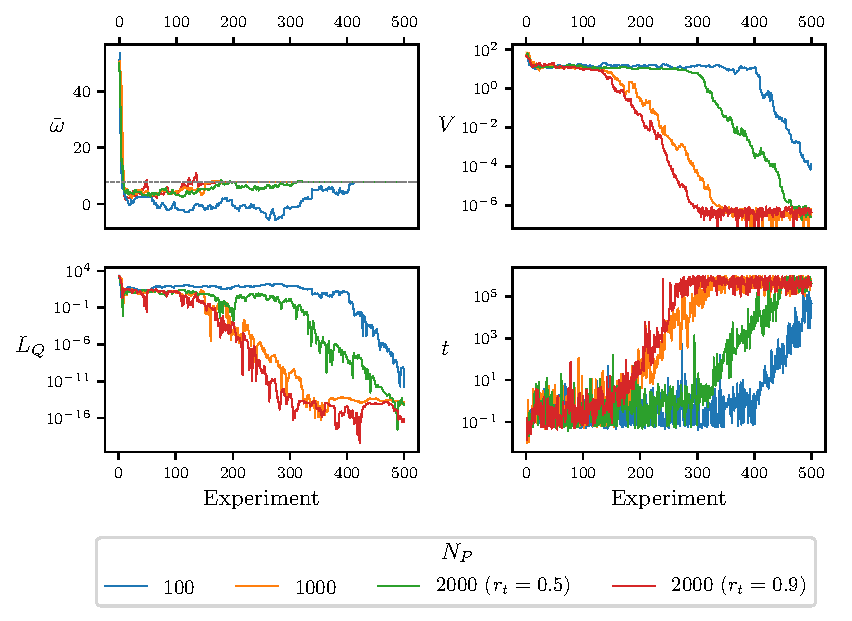
\includegraphics{algorithms/figures/params.pdf}
    \caption[Parameter learning varying number of particles]{
        Parameter learning for the analyitcal likelihood \cref{eqn:analytical_likleihood}
        for varying numbers of particles $\Np$, for $\Ne=500$. 
        For $\Np=2000$, we show the resampler threshold set to $r=0.5$ and $r=0.9$. 
        (a) the parameter estimate, i.e. $\bar{\omega}$, the mean of the posterior distribution after each experiment, 
        approaching $\omega_0=7.75$ (dashed line), where the prior is centred on $\omega=50 \pm 25$. 
        Decrease in (b) volume, $V$, (c) quadratic loss, $L_Q$, 
        and (d) evolution time, $t$, are shown against experiment number.
    }
    \label{fig:param_learning_vary_particles}
\end{figure}


\gls{qhl} is a parameter estimation algorithm, so here we introduce some methods to evaluate its performance, 
    which we can reference in later sections of this thesis. 
\par 
The most obvious meausre of the progression of parameter estimation is the error between the true parameterisation, 
    $\al_0$, and the approximation $\al_p = \mean \bk{ \Pr(\al) }$,
    which can be captured by a large family of loss functions. 
Here we use the \gls{ql}, which captures this error through the sum of the square difference between 
    each parameter's true and estimated values symetrically, 
    i.e. error above the true parameter is as impactful as error below. 
We can record the \gls{ql} at each experiment of our training regime and hence track its performance. 
\begin{definition}[Quadratic Loss]
    \label{def:quadratic_loss}
    For a true parameterisation $\al_0$, and a hypothesis $\al$, the quadratic loss is given by
    \begin{equation}
        \label{eqn:quadratic_loss}
        L_{Q} = \left\| \al_0 - \al \right\|^2.
    \end{equation}
\end{definition}
\par 

\subsection{Volume}\label{sec:volume}
We also care about the range of parameters supported by $\Pr(\al)$ at each experiment: 
    the \gls{volume} of the particle distribution can be seen as a proxy for our certainty
    that the approximation $\mean\bk{\Pr(\al)} $ is accurate. 
For example, for a single parameter $\omega$, our best knowledge of the parameter is $\mean\bk{ \Pr(\omega) }$, 
    and our belief in that approximation is the standard deviation of $\Pr(\omega)$; 
    we can think of volume as an $n$-dimensional generalisation of this intuition \cite{qinfer-1_0, ferrie2014high}. 
\par 
In general, a confidence region, defined by its confidence level $\kappa$, is drawn by grouping particles 
    of \gls{hpd}, $\mathcal{P}$, such that $\sum\limits_{p \in \mathcal{P}} w_{p} \geq \kappa$.
We use the concept \todo{do we use MVEE or the posterior directly as the credible region?} of \gls{mvee} 
    to capture the confidence region \cite{ferrie2014high}, calculated as in \cite{todd2007khachiyan}, 
    which are characterised by their covariance matrix, $\Sigma$, which allows us to calculate the \gls{volume}, 
    \begin{equation}
        \label{eqn:volume}
        V(\Sigma) = \frac{ \pi^{| \al | / 2}}{ \Gamma(1 + \frac{| \al |}{2})} \det\bk{\Sigma^{-\frac{1}{2}}},
    \end{equation}
    where $\Gamma$ is the Gamma function, and $|\al|$ is the cardinality of the parameterisation. 
This quantity allows us to meaningfully compare distributions of different dimension, 
    but we must be cautious of drawing strong comparisons between models based on 
    their volume alone, for instance because they may have started from vastly different prior distributions. 
\par 

Within \gls{smc}, we assume the credible region is simply the posterior distribution, 
    such that we can take $\Sigma = \textrm{cov}(\Pr(\al))$ after each experiment, 
    and hence track the uncertainty in our parameters across the training experiments \cite{Granade:2012kj}.
We use volume as a measure of the learning procedure's progress: 
    slowly decreasing or static volume indicates poor learning, possibly highlighting poor experiment design, 
    while fast or exponentially decreasing volume indicates that the parameters are being learned well. 
When the volume has converged, the learning has saturated and there is little benefit to running further experiments. 

\section{Experiment design heuristic}
\label{sec:heuristic}
A key consideration in \gls{qhl} is the choice of experimental controls implemented in attempt to learn from the system. 
The experimental controls required are dictated by the choice of \gls{likelihood} function used within \gls{smc}, 
    though typically there are two primary controls we will focus on: 
    the evolution time, $t$, and the \gls{probe} state evolved, $\ket{\psi}$. 
The design of experiments is handled by an \gls{edh}, 
    whose structure can be altered to suit the user's needs. 
Usually, the \gls{edh} attempts to exploit the information available, 
    adaptively accounting for some aspects of the inference process performed already, 
    although there may be justification for enforcing a non-adaptive schedule, 
    for instance to force \gls{qhl} to train on a full set of experimental data 
    rather than a restricted set which adaptive methods would advise.
We can categorise each \gls{edh} as either \emph{online} of \emph{offline},
    depending on whether it accounts for the current state of the inference procedure, i.e. the posterior.
The \gls{edh} is modular and can be replaced by any method that returns a valid set of experimental controls, 
    so we can consider numerous approaches, for instance those described in \cite{hincks2018hamiltonian, fiderer2020neural}.
\par 

\subsection{Particle Guess Heuristic}\label{sec:pgh}
The default \gls{edh} is the \gls{pgh} \cite{Wiebe:2014qhl}, 
    an online method which attempts to design the optimal evolution time based on the posterior.
Note \gls{pgh} does not specify the \gls{probe}, so is coupled with a \gls{probe} selection routine to comprise 
    a complete \gls{edh}.
\par

The principle of \gls{pgh} is that the uncertainty of the posterior limits how well the Hamiltonian is currently 
    approximated, and therefore limits the evolution time for which the posterior can be expected to 
    reasonably mimic $\ho$.
For example, consider \cref{eqn:analytical_hamiltonian} with a single parameter with $\omega_0 = 10$,
    and current $\mean\bk{\Pr(\omega)} = 9, \std\bk{\Pr(\omega)} = 2$, 
    we can expect that the approximation $\omega^{\prime} = \mean\bk{\Pr(\omega)}$ 
    is valid up to $t_{max} = \nicefrac{1}{\std\bk{\Pr(\omega)}}$. 
% TODO make a figure illustrating this point with some wide, medium and thin priors
It is sensible, then, to use $t \sim t_{max}$ for two reasons: 
    (i) smaller times are already well explained by the posterior, so offer little opportunity to learn;
    (ii) $t_{max}$ is at or near the threshold the posterior can comfortably explain, 
        so it will expose the relative difference in likelihood between the posterior's particles, 
        providing a strong capacity to learn. 
Informally, as the uncertainty in the posterior shrinks, \gls{pgh} selects larger times 
    to ensure the training is based on informative eperiments simulataneously with increasing 
    certainty about the paraemters. 
In the one-dimensional case, this logic can be used to find an optimal time heuristic, 
    where experiment $k$ is assigned $t_k = \nicefrac{1.26}{\std\bk{\Pr(\omega)}}$ \cite{ferrie2013best}. 
\par
Rather than directly using the inverse of the standard deviation of $\pr{\al}$, 
    which relies on the expensive calculation of the covarinace matrix, 
    \gls{pgh} uses a proxy whereby two particles are sampled from $\pr{\al}$. 
The experimental evolution time for experiment $k$ is then given by 
\begin{equation}
    \label{eqn:pgh_time}
    t_k = \frac{1}{\| \al_i - \al_j \|}, 
\end{equation}
    where $\al_i, \al_j$ are distinct particles sampled from $\mathcal{P}$ where 
    $\mathcal{P}$ is the set of particles under consideration by \gls{smc} after experiment $k-1$, 
    which had been recently sampled from $\Pr\bk{\al}$. 
\par 


\subsection{Alternative experiment design heuristics}\label{sec:alt_heuristics}
The \gls{edh} can be used to suit the requirements of the target system; 
    we test four such examples against a series of models. 
Here the \gls{edh} must only design the evolution time for the experiment, 
    with probe design discussed in the next section. 
The heuristics tested are:

\begin{easylist}
    \ListProperties(Numbers=r)
    & $\textrm{Random}(0, t_{max})$: Randomly chosen time up to some arbitrary maximum, we set $t_{max} = 1000$. 
        This approach is clearly subobtimal, since it does not account whatsoever for the knowledge of the training so far, 
        and demands the user choose a suitable $t_{max}$, which is not gauranteed to be meaningful. 
    & $t$ list: forcing the training to consider a set of times decided in advance.
        For instance, when only a small set of experimental measurements are available, it is sensible to train on all of them, perhaps repeatedly. 
        We test uniformly spaced times between 0 and $t_{max}$, and train on the list twice.
        Again this \gls{edh} fails to account for the performance of the trainer so far, so may use times either 
        far above or below the ability of the parameterisation. 
    & $(\nicefrac{9}{8})^k$: An early attempt to match the expected exponential decrease in volume from the training, 
        was to set $t = (\nicefrac{9}{8})^k$ \cite{Granade:2012kj}.
        Note we increment $k$ after 10 experiments in the training regime, 
        rather than after each experiment, which would result in extremely high times which flood memory.
    & \Gls{pgh}: as in \cref{sec:pgh}. 
\end{easylist}

We show how the choie of \gls{edh} within this set can influence the training procedure,
    by testing models of various complexity amd dimension. 
In particular, we first test a simple 1-qubit model, \cref{eqn:qhl_test_model_1}; 
    followed by more complicated 1-qubit model, \cref{eqn:qhl_test_model_2};
    as well as randomly generated 5-qubit Ising, \cref{eqn:qhl_test_model_3}, and 4-qubit Heisenberg models, \cref{eqn:qhl_test_model_4}.
Each $\hi$ have randomly chosen parameters implicitly assigned to each term. 
\begin{subequations}\label{eqn:qhl_test_models}
    \begin{equation}
        \label{eqn:qhl_test_model_1}
        \h_1=\s^z_1
    \end{equation}
    \begin{equation}
        \label{eqn:qhl_test_model_2}
        \h_2 = \s^x_1 + \s^y_1 + \s^z_1
    \end{equation}
    \begin{equation}
        \label{eqn:qhl_test_model_3}
        \h_3 = \s^z_1\s^z_3 + \s^z_1\s^z_4 + \s^z_1\s^z_5 + \s^z_2\s^z_4 +\s^z_2\s^z_5 + \s^z_3+\s^z_4 + \s^z_3+\s^z_5
    \end{equation}
    \begin{equation}
        \label{eqn:qhl_test_model_4}
        \h_4 = \s^z_1\s^z_2 + \s^z_1\s^z_3 +\s^x_2\s^x_3 + \s^z_2\s^z_3 + \s^x_2\s^x_4 + \s^z_3\s^z_4
    \end{equation}
\end{subequations}

\begin{figure}
    \begin{center}
        \QMLAfig{Nov_27/heuristic_comparisons.pdf}
    \end{center}
    \caption[Training with different heuristics]{
        The volume of various models when trained through \gls{qhl} using different \glspl{edh}.
        We show models of various complexity and dimension, each trained using four heuristics, 
        outlined in the main text.
        \figtableref
    }
    \label{fig:heuristics_test}
\end{figure}

We show the performance of each of the listed \glspl{edh} in \cref{fig:heuristics_test}. 
We will have cause to use alternative \glspl{edh} in paricular circumstances, 
    but we adopt \gls{pgh} as the default \gls{edh} throughout this thesis, 
    unless otherwise stated.


\section{Probe selection}

A final consideration for experiments within \gls{qhl} is the choice of input \gls{probe} state, $\ket{\psi}$,
    which is evolved in the course of finding the likelihood used during the Bayesian update. 
We can consider the choice of probe as an output of the \gls{edh},  
    although previous work has usually not considered optimising the \gls{probe}, 
    instead usually setting $\ket{\psi} = \ket{+}^{\otimes n}$ for $n$ qubits \cite{wang2017experimental, ferrie2013best}.
In principle it is possible for the \gls{edh} to design a new \gls{probe} at each experiment, 
    although a more straightforward approach is to compose a set of probes offline, $\Psi = \{ \ket{\psi} \}$,
    of size $\Npsi = \absval{\Psi}$.
Then, a probe is chosen at each experiment from $\Psi$, 
    allowing for the same $\ket{\psi}$ to be used for the multiple experiments within the training, e.g. by iterating over $\Psi$. 
$\Psi$ can be generated with respect to the individual learning problem as we will examine later, 
    but it is usually sufficient to use generic strategies which should work for all models;
    some straightforward examples are
    \begin{easylist}[enumerate]
        \ListProperties(Numbers=r)
        & $\ket{0} : \ \Psi = \{\ket{0}^{\otimes n}\}, \ \ \Npsi=1$;
        & $\ket{+} : \ \Psi = \{\ket{+}^{\otimes n}\}, \ \ \Npsi=1$;
        & $\ket{t} : \ \Psi$ is the tomographic basis set, \ \ $\Npsi=40$;
        & $\ket{r} : \ \ket{\psi}$ are random, separable probes, \ \ $\Npsi=40$.
    \end{easylist}
\par 
We show the 1-qubit probes within $\Psi$ under each of these strategies on the Bloch sphere in \cref{fig:probes_used_bloch}.

\begin{figure}
    \begin{center}
        \subfloat{
            % 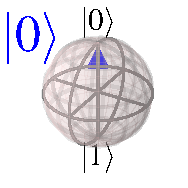
\includegraphics[width=0.2\textwidth]{qmla_run_data/Nov_27/zero_probes.pdf}
            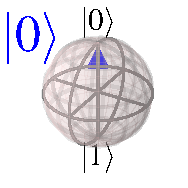
\includegraphics{qmla_run_data/Nov_27/zero_probes.pdf}
        }
        \qquad
        \subfloat{
            % 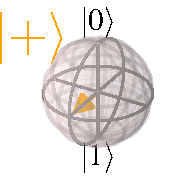
\includegraphics[width=0.2\textwidth]{qmla_run_data/Nov_27/plus_probes.pdf}
            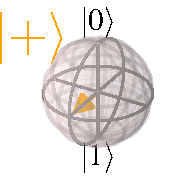
\includegraphics{qmla_run_data/Nov_27/plus_probes.pdf}
        }
        \qquad
        \subfloat{
            % 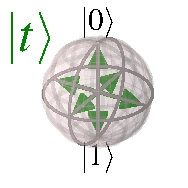
\includegraphics[width=0.2\textwidth]{qmla_run_data/Nov_27/tomographic_probes.pdf}
            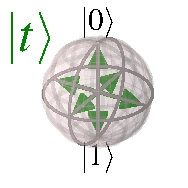
\includegraphics{qmla_run_data/Nov_27/tomographic_probes.pdf}
        }
        \qquad
        \subfloat{
            % 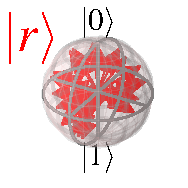
\includegraphics[width=0.2\textwidth]{qmla_run_data/Nov_27/random_probes.pdf}
            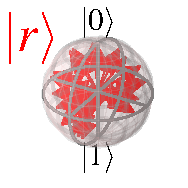
\includegraphics{qmla_run_data/Nov_27/random_probes.pdf}
        }
        \qquad
    \end{center}
    \caption[Probes used for tests]{
        1-qubit probes used for tests in \cref{fig:probes_test}.
    }
    \label{fig:probes_used_bloch}
\end{figure}

\begin{figure}
    \begin{center}
        \QMLAfig{Nov_27/training_probes.pdf}
    \end{center}
    \caption[Training with different probes]{
        The volume of various models when trained through \gls{qhl} using different initial \gls{probe} sets. 
        We show models of various complexity and dimension, each trained using random probes, $\ket{r}$, 
        tomographic basis set probes, $\ket{t}$, as well as $\ket{0}$ and $\ket{+}$ probes. 
        In each case the probes are generated for arbitrary numbers of qubits; 
        for $\ket{0}, \ket{1}$, the number of probes generated is $N_{\psi}=1$, 
        and for $\ket{t}, \ket{r}$, $N_{\psi}=40$.
        \figtableref
    }
    \label{fig:probes_test}
\end{figure}

We test the same set of models as \cref{eqn:qhl_test_models} and test each of these \gls{probe} construction 
    strategies in \cref{fig:probes_test}. 
We can draw a number of useful observations from these simple tests: 
\begin{easylist}[itemize]
    & Training on an eigenstate, $\ket{0}$, of the model yields no information gain. 
        This is because all particles give likelihoods $l=1$, 
    so no weight update can occur, meaning the parameter distribution does not change when presented new evidence. 
    & Training on an even superposition of the model's eigenstates, $\ket{+}$, is maximally informative: 
        any deviations from the true parameterisation are registered most dramatically in this basis,
        providing the optimal training probe for this case.     
    & These observations are reinforced by \cref{fig:probes_test}\textbf{c}, where a 5-qubit Ising model also 
        fails to learn from one of its eigenstates, $\ket{0}^{\otimes 5}$.
        Of note, however, is that $\ket{+}^{\otimes 5}$ is not the strongest probe here: the much larger Hilbert space here 
        can not be scanned sufficiently using a single probe; 
        using a larger number of probes is more effective, even if those are randomly chosen. 
    & In general the tomographic and random probe sets perform reliably. 
\end{easylist}

It is an open challenge to identify the optimal probe for training any given model, 
    and the choice of such informative probes could be built into the \gls{edh} in general, 
    for example by computing the eigenstates of the candidate, and generating a probe set
    from superposition between those eigenstates. 
However, a further consideration is that, for model comparison purposes, 
    it is helpful to have a universal set of probes, upon which all models are learned. 
This would minimise bias towards particlar models, which might arise from probes which are favourable bases 
    for a subset of models, for example $\ket{+}$ in \cref{fig:probes_test}\textbf{a}. 
Careful consideration should be given to $N_{\psi}$ in the choice of the probe generator, 
    since it is important to ensure probes test the parameterisation across the Hilbert space robustly, 
However this must be balanced by ensuring \gls{smc} has sufficient opportunity to learn within a subspace before moving to the next; 
    we can mitigate this concern by instructing the \gls{edh} to repeatedly select a probe from $\Psi$ for a batch of experiments, 
    say five, before moving to the next available probe. 
\par 

As standard for the remainder of this thesis, unless otherwise stated, 
    we adopt the random probe generator as the defualt mechanism for selecting probes,
    only iterating between probes after batches of 5 experiments.
